\section{System Overview}\label{sec:system}
\begin{alltt}\scriptsize
- System overview
    - How interaction graph are currently stored
        - Most of the disk space work is on regular graphs, 
           not interaction graphs. 
        - Approach this as this is the railway, and we built
           on this prior work.
        - Builds on existing work that does not support 
          adaptivity.
    - Introduce the rail layout
    - Add the figure
    - Query model
   - Note that we need to talk here:
    - For the system implementation, we need to add an additional
       index to have a list of partitions for a block
   - We also need to know how attributes are partitioned across sub-blocks 
      for a given time interval.

    - Current layout:
    head vertex (id), num items in neighbor list, 
    for each entry:
        timestamp of edge
        id of other edge of vertex
        any edge properties

\end{alltt}


\begin{figure}[ht!]
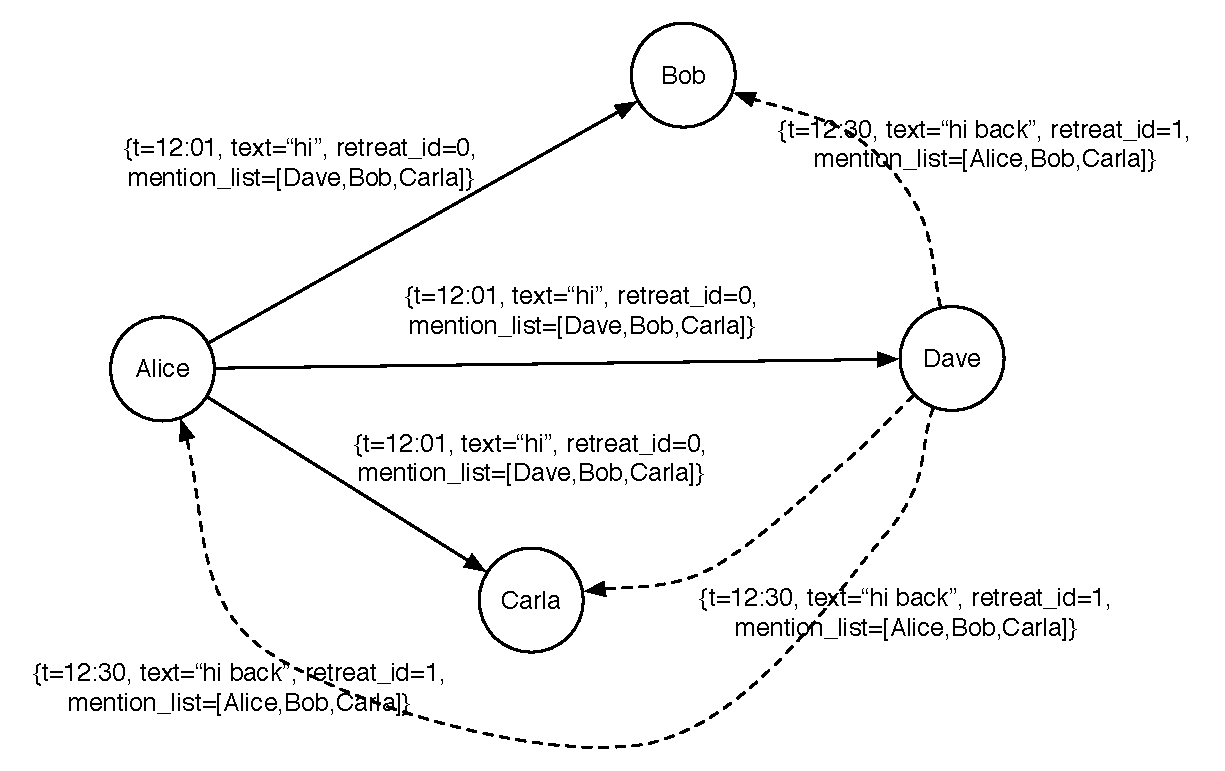
\includegraphics[width=0.33\textwidth]{figures/example_interaction.pdf} 
 \caption{An example interaction graph for a small social network.}
 \label{fig:example}
 \end{figure}